\documentclass[conference]{IEEEtran}
\usepackage{graphicx}
\graphicspath{{Figures/}}

\begin{document}
	\title{I am a title (RO SLAM Methods/Implementation Survey) }

	\author{David Grabowsky}
	
	\markboth{IEEE Transactions On xxxl, Vol. XX, No. Y, Month 2018}{Grabowsky: RO SLAM}
	
	
	
	\maketitle
	
	
\begin{abstract}

	
	This is my abstract, there are many like it, but this one is mine. Will fill this in once paper is written ****
	
	An survey of current the current implementations and methodologies used for solving the range only systematic and localization problem (RO-SLAM). 

\end{abstract}
	
	
	
\section{Introduction} 

\section{range only sensors/tech}
\section{Methods...}
\subsection{EKF}
%breif description (1-2 paragraphs)
%paragraphs 
The Extended Kalman Filter (EKF) is one of the most popular and widespread methods used to solve the SLAM problem. It is used to overcome the assumption of linear state transitions and measurements, which are rarely seen in practical environments \cite{Thrun2002}. The derivation of the EKF is very well documented, as such, detailed explanations can be viewed from a variety of sources such as: \cite{Thrun2002}, \cite{Ribeiro2004}, and \cite{Haykin2001}. When used to solve SLAM the map applied to the EKF is a feature based map, meaning it is composed of observable features (landmarks) which can be distinguished between during re-observation.\cite{Thrun2002} This distinction becomes important when examining range only SLAM (RO-SLAM) where only the range to a landmark, or the range between landmarks, is known. This restriction means that landmarks often need to be manufactured, such as those discussed in section II, and physically placed in an environment. Landmark initialization is a critical element in many algorithms that make use of the EKF. If the initialization is inaccurate then the convergence to a correct estimation becomes more difficult. 

A system for robust range only localization was prosed by Olson \cite{Olson2006}. The system utilized an Autonomous Underwater Vehicle (AUV) and beacons without carefully surveyed locations. A method for outliers rejection was accomplished via spectral graph partitioning. A voting scheme was implemented similar to a Hugh transform to get approximate beacon locations \cite{Hough1959}. The approximate location was then incorporated into an EKF. The methodology was simulated using a dataset from the GOAT'02 experiment and can be seen in the report. %get a citaion for goat.


Multipathing and noise presents major obstacle to any radio frequency based RO-SLAM solutions. Research and experimentation has been conducted to determine how these effects can be mitigated without the use of specialized equipment. Fabresse presents a pre-filtering algorithm to be applied to range measurment before being used in the EKF in order to reduce these effects \cite{Fabresse2014}. The author also validates and expands upon this method through indoor and outdoor experimentation with an Unmanned Aircraft System (UAS). \cite{Fabresse2016}. 

%fabreese. 
%1. 2013 presents EKF slam method for ariel vehicles 
%2. 2014 introduces prefiltering to measurments for previous 
%3. 2014a integrates visual landmakrs as well
%4  2015 decentralized multiple arieal vehicles
%5  2016 specifically unmaned ariel, more details on 2013,2014 and experimental validation of 2013,2014.

Vallicrosa presents a solution utilizing a Sum of Gaussian (SOG) filter for a single range only beacon. The filter made use of the EKF by representing each Gaussian in the SOG as a complete EKF \cite{Vallicrosa2015}. Results are given from a simulated environment.

Several techniques have also been implemented that involve cooperative sensors. The sensors in these cases are able to determine the range between themselves and other sensors and or the robot \cite{Patwari2005}.

\begin{figure}[h!]
	\centering
	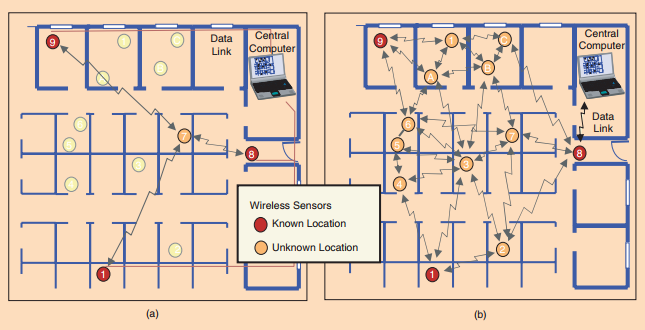
\includegraphics[width=90mm]{coop_loc_comp_patwari.png}
	\caption{Traditional(a) vs Cooperative(b) Sensors \cite{Patwari2005}}
	\label{trad_vs_coop_sensors}
\end{figure}

%ADD MORE HERE
In scenarios where the location of the landmarks is unknown and each landmark can not communicate with all other landmarks, Djugash presents a solution. He proposes that a moving beacon be used to add edges to the network \cite{Djugash2006}. In addition, no external position sensing were required on the part of the moving beacon, but the option for it to be incorporated was available. 

Torres-Gonzalez explains that methods utilizing inter beacon measurment should incorporate measurements with a configurable number of hops between beacons. This allows for the robot to gather range data from beyond the extent of the robots sensors \cite{Torres-Gonzalez2015}. Based on testing with an EKF, his results showed that the more hops that were added the greater the performance of the system. 

One of the complications with RO-SLAM involves the issue of determining the location of landmarks when their initial placement is unknown, the EKF is sensitive to poorly initialized landmarks as they are used as the basis for the convergence of an accurate estimate. Caballero presents a solution for this complication. \cite{Caballero2010}. A Gaussian Mixture Model is integrated into the EKF to create a multiple hypothesis filter.  This multiple hypothesis approach is used to solve the RO-SLAM problem and its use allows for the un-delayed initialization of landmarks, however a large number of hypothesis can lead to increased computational burden. Geneve
%fix the name
also puts forward a method that utilizes a Gaussian mixtures for beacon initialization in EKF, but in this method only two hypotheses and a Cartesian plane are used \cite{Geneve2015}.  Ahmad proposes to reduce the computational burden of methods such as the one proposed by Caballero \cite{Caballero2010} by introducing a novel state vector that eliminates the need for multiple hypothesis landmark representation. The paper proposes that under different circumstances the landmark could be represented using different parameters  \cite{Ahmad2011a}. Four circumstances are presented in the paper and the method is tested in simulation using both the EKF and a least squares optimization approach. The results showed that when the circumstances can be clearly distinguished between an increase in performance is seen.

Djugash proposes an extension to EKF called relative-over parametrized (ROP) EKF. This extension uses specific parameterization to  better represent the range only data utilized in RO-SLAM. \cite{Djugash2008}. ROP EKF operates in polar coordinates as opposed to the Cartesian space that typical EKF operates.
\begin{figure}[h!]
	\centering
	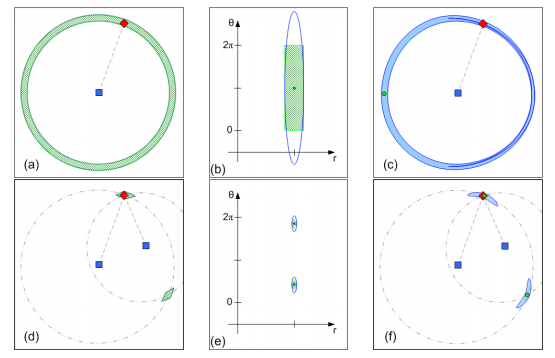
\includegraphics[width=90mm]{ROP_djugash.png}
	\caption{True and approximated distributions with one range observation (Top Row) and two observations from different locations (Bottom Row). True distributions in	Cartesian coordinates (Left Column), true and Gaussian approximated distributions in polar coordinates (Middle Column), and projection of the Gaussian approximated. \cite{Djugash2008}} %THIS WAS LITTERALY COPYIED AND PASTED AND NEEDS TO BE CHANGED AT SOME POINTS
	\label{ROP_djugash}
\end{figure}


The method provided improved results over EKF when sparse range measurement of data association errors were present. Herranz presents a comparison of the ROP-EKF method presented by Djugash \cite{Djugash2008},to a smoothing and mapping method presented by Dellaert \cite{Dellaert2006}. Experimentation conducted by Herranz on and indoor and outdoor environment show an improvement in the results of the SAM method over ROP EKF. \cite{Herranz2014}

A method proposed by \cite{Dios2015} is geared towards improving map building speed and accuracy for UAS dealing with the 3D RO-SLAM problem. The 3D RO-SLAM problem refers to the added complexity that devices such as submersibles \cite{Newman} and aerial vehicles experience when having to operate in an environment where three dimensions must be considered as opposed to the planar environment many robots are assumed to operate in. The method utilizes inter-beacon measurements and a novel mode selection which is used to select a measurement gathering method based on current conditions \cite{Dios2015}.
%this one might need some more work

\cite{Fabresse2013} presents a solution for the 3D RO-SLAM problem. The solution reduces computational load through reduced spherical parametrization of map feature positions. The paper also proposes a new EKF update method which incorporates a reduced spherical representation of the state vector. In addition the paper describes how to efficiently integrate multi-modal belief of elevations angles and azimuth from a range sensor into the EKF utilizing two independent Gaussian Mixtures \cite{Fabresse2013}. It is proposed by \cite{Fabresse2015} that the above method can be utilized for decentralized multi-SLAM with range only sensors. This new method would allow for landmarks estimated by a robot to be incorporated into the estimation of another nearby robot, thus improving localization estimation. 




%2015 (decentrailzied) works off 2013 (undelayed)


\subsection{Graph SLAM}
\subsection{Particle}
\subsection{Graph}
\subsection{Fast}

\section{Conclusion}


	\bibliographystyle{IEEEtran}
	\bibliography{references}
	
\end{document}

